
\section{Squares for Unordered Alphabets}
\newcommand{\absolute}[1]{\left\lvert#1\right\rvert}
\newcommand{\orderof}[1]{\mathcal{O}(#1)}

\begin{frame}
    \centering
    {\Large Optimal Square Detection  Over General Alphabets}
  
    \bigskip
    {\large SODA'23}\\
    \bigskip
    
\includegraphics{pictures/mindmap/squares.png}
  
    \bigskip
    Jonas Ellert, Paweł Gawrychowski
\end{frame}




\begin{frame}{Squares and repetition detection}

    \vspace{1.5\baselineskip}
    \noindent%
    \begin{tikzpicture}[x = 2em, remember picture]
    \foreach[count=\i from 1, evaluate=\i as \pos using int(\i - 1)] \x in {m,i,s,s,i,s,s,i,p,p,i} {
    \node<1> (\i) at (\pos, 0) {\smash{\texttt\x}$\vphantom{m}$};
    \node<2->[color=white] (\i) at (\pos, 0) {\smash{\texttt\x}$\vphantom{m}$};
    \node<2-> (s1-\i) at (\pos, 0) {\smash{\texttt\x}$\vphantom{m}$};
    }
    
    %\foreach[count=\i from 1, evaluate=\i as \pos using int(\i - 1)] \x in {,i,s,s,i,s,s,,,,} {
    %\node (s1-\i) at (\pos, 0) {\smash{\texttt\x}$\vphantom{m}$};
    %}
    
    \foreach[count=\i from 1, evaluate=\i as \pos using int(\i - 1)] \x in {,,s,s,i,s,s,i,,,} {
    \node<5->[color=gray] (s2-\i) at (\pos, -.6) {\smash{\texttt\x}$\vphantom{m}$};
    }
    
    \foreach[count=\i from 1, evaluate=\i as \pos using int(\i - 1)] \x in {,,s,s,,s,s,,p,p,} {
    \node<6->[color=gray] (s3-\i) at (\pos, -1.2) {\smash{\texttt\x}$\vphantom{m}$};
    }
    
    \path<3-> (4) to node[midway, above=2.1em] {$\overbrace{\phantom{aaaaaaaaaaaaaaaaaaaaa}}^{\displaystyle\text{square of period $3$}}$} (5);
    
    \path<4-> (3) node[above=.25em] {$\overbrace{\phantom{aaaaaaaaaa}}^{\displaystyle\text{left arm}}$};
    \path<4-> (6) node[above=.25em] {$\overbrace{\phantom{aaaaaaaaaa}}^{\displaystyle\text{right arm}}$};
    
    \draw<-6> (11) node[right=2.5em] {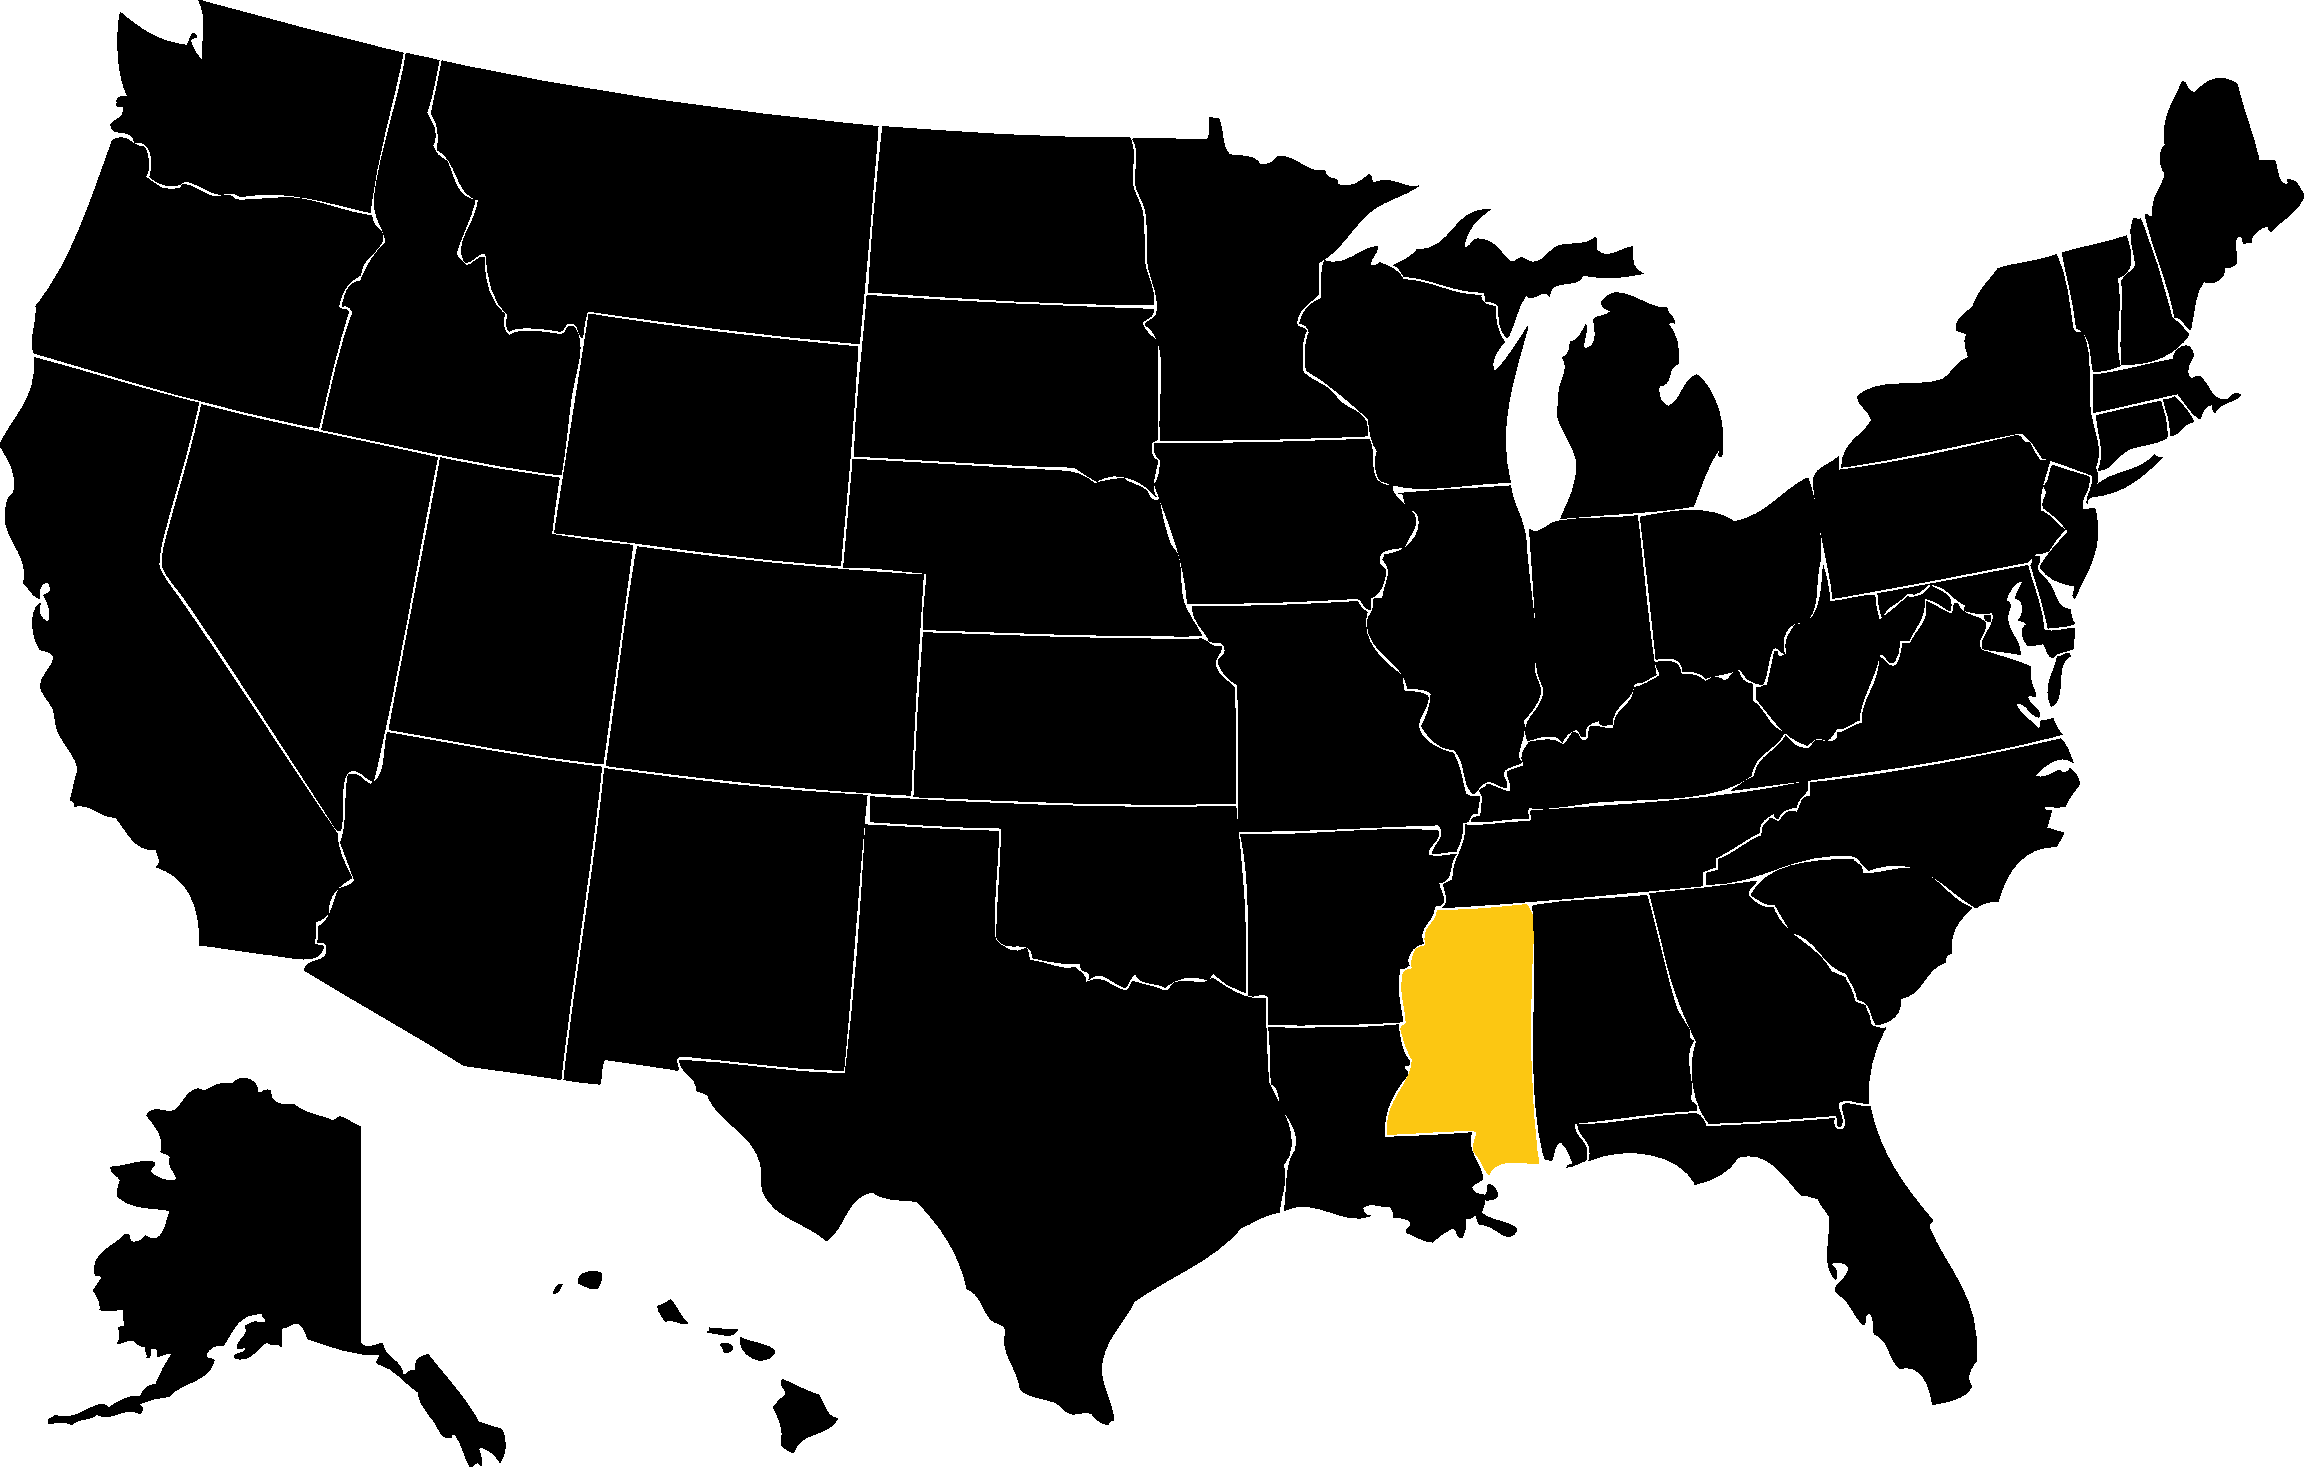
\includegraphics[scale=0.15]{pictures/mississippi.pdf}};
    \draw<7-> (11) node[right=2.5em] {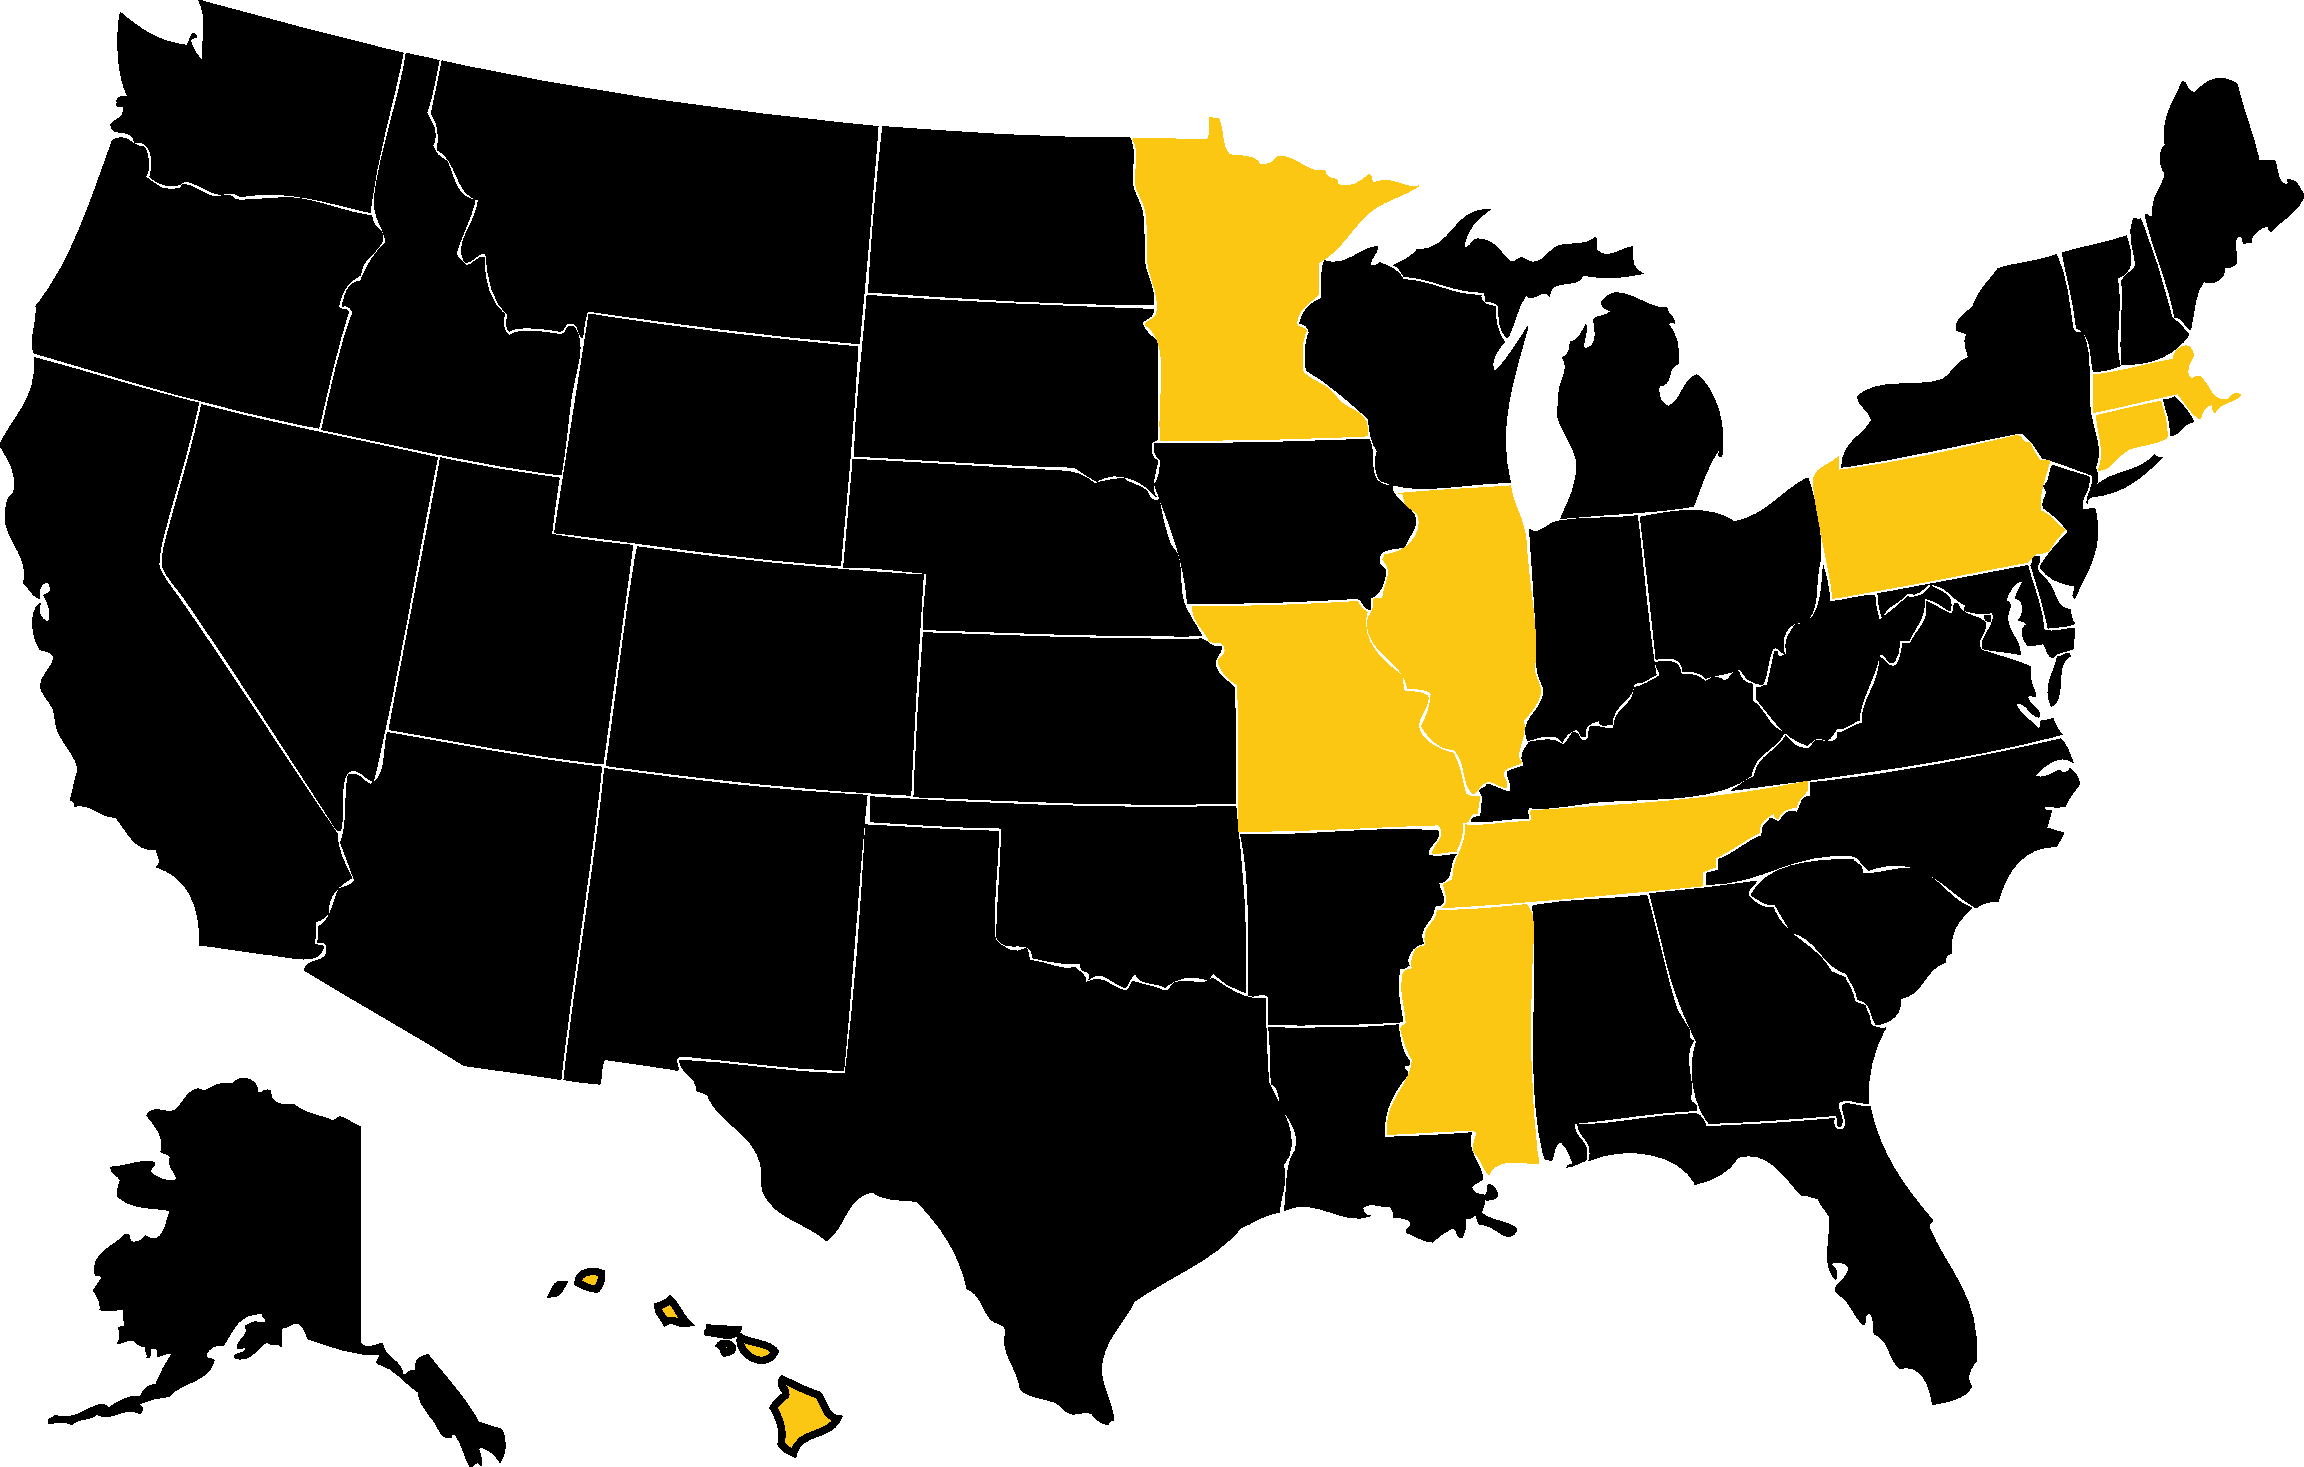
\includegraphics[scale=0.15]{pictures/square-states.pdf}};
    \draw<7-> (11) node[below right=5.5em and 3em] {\tiny{Connecticut, Hawaii, Illinois, Massachusetts, Minnesota, Mississippi,}};
    
    \path (1.south) ++(0,.25em) node (v0) {};
    \path (v0) ++(0,-.5em) node (v1) {};
    \path (v1) ++(0,-.5em) node (v2) {};
    \path (v2) ++(0,-.5em) node (v3) {};
    \path (v3) ++(0,-.5em) node (v4) {};
    \path (v4) ++(0,-.5em) node (v5) {};
    
    \draw<2->[ultra thick, myorange] (s1-2.north west) rectangle (s1-4.south east);
    \draw<2->[ultra thick, myorange] (s1-5.north west) rectangle (s1-7.south east);
    
    \draw<5->[ultra thick, mygreen] (s2-3.north west) rectangle (s2-5.south east);
    \draw<5->[ultra thick, mygreen] (s2-6.north west) rectangle (s2-8.south east);
    
    \draw<6->[ultra thick, myred] (s3-3.north west) rectangle (s3-3.south east);
    \draw<6->[ultra thick, myred] (s3-4.north west) rectangle (s3-4.south east);
    
    \draw<6->[ultra thick, myred] (s3-6.north west) rectangle (s3-6.south east);
    \draw<6->[ultra thick, myred] (s3-7.north west) rectangle (s3-7.south east);
    
    \draw<6->[ultra thick, myblue] (s3-9.north west) rectangle (s3-9.south east);
    \draw<6->[ultra thick, myblue] (s3-10.north west) rectangle (s3-10.south east);
    
    
    \end{tikzpicture}
    
    \flushleft
    
    %\vspace{\baselineskip}
    
    
    \onslide<8->{\textcolor<11->{gray}{\textbf{Some problems regarding squares:}}}
    
    \begin{itemize}
    \item<8->\textbf<11->{test square-freeness, i.e., whether or not a word contains a square}
    \item<9->\color<11->{gray} compute all squares (or runs) in a given word
    \item<10->\color<11->{gray} compute all distinct squares in a given word
    \end{itemize}
\end{frame}


\begin{frame}{Alphabet types for $w \in \Sigma^n$, where $|\Sigma| = \sigma$}
    \small
	\vspace{.75\baselineskip}	
	
	\setlength{\leftmargini}{1.1em}
	\begin{itemize}
	\onslide<2->{\item \textbf{linearly-sortable alphabet (LSA)}:\hfill \hspace{0.5cm}%
	\onslide<3->{e.g.\ $\{\texttt A,\texttt C,\texttt G,\texttt T\}$, $\{0, \dots, 255\}$, or $\{1, \dots, n^{\Oh({1})}\}$}
	\\sort $n$ symbols in $\Oh({n})$ time%\\e.g.\ $\{1, \dots, n^{\Oh{1}}\}$%
	}
	\vspace{.25\baselineskip}
	\onslide<4->{\item \textbf{general ordered alphabet (GOA)}:\hfill %
	\onslide<5->{\rlap{e.g.\ comparison sort}\phantom{e.g.\ $\{\texttt A,\texttt C,\texttt G,\texttt T\}$, $\{0, \dots, 255\}$, or $\{1, \dots, n^{\Oh{1}}\}$}}
	\\test $w[i] < w[j]$ in constant time}
	\vspace{.25\baselineskip}
	\onslide<6->{\item \textbf{general unordered alphabet (GUA)}:\hfill%
	\onslide<7->{\rlap{e.g.\ KMP pattern matching}\phantom{e.g.\ $\{\texttt A,\texttt C,\texttt G,\texttt T\}$, $\{0, \dots, 255\}$, or $\{1, \dots, n^{\Oh{1}}\}$}}
	\\test $w[i] = w[j]$ in constant time}
	\end{itemize}
	
	\vspace{1.5\baselineskip}
	\onslide<8->
	\begin{tabular}{r|ccc} 
		& LSA & GOA & GUA \\\hline
		%${}^{\strut}$Element Distinctness & $\Theta(\sigma)$ & $\Theta(\sigma \lg \sigma)$ & $\Theta(\sigma^2)$ \pause \\
		$\strut^{\strut}$Lempel-Ziv & %
		\onslide<9->{$\Oh({n})$} & %
		\onslide<10->{$\Theta(n \lg \sigma)$} & %
		\onslide<11->{$\Theta(n\sigma)$} \\ %
		%
		$\strut$Suffix Sorting & %
		\onslide<9->{$\Oh({n})$} & %
		\onslide<10->{$\Theta(n \lg \sigma)$} & %
		\onslide<11->{$\Theta(n\sigma)$} \\
		%
		\onslide<12->{${}^{\strut}$\bfseries Square-Freeness} & %
		\onslide<12->{\boldmath$\Oh({n})$\unboldmath} & %
		\onslide<13->{\boldmath$\Theta(n)$\unboldmath} & %
		\onslide<14->{\boldmath$\Oh(n \lg n)$\unboldmath} \begin{tikzoverlay}
			\onslide<15->{
            \beamermathcolor{black}
			\tikzset{viscol1/.style={white}}
			\tikzset{viscol2/.style={white}}
			\tikzset{viscol3/.style={white}}
			\only<16->{\tikzset{viscol1/.style={}}}
			\only<17->{\tikzset{viscol2/.style={}}}
			\only<17->{\tikzset{viscol3/.style={red}}}
			\path (0,.1) node (a) {};
			\draw (3,1.1) node (b) {optimal for $\sigma = n$};
			\node[below=-.4em of b,viscol1] (c) {but what about $\sigma < n\strut$?};
			\node[below=-.0em of c,viscol2] (d) {{\boldmath$\Theta(n \lg \sigma)$\unboldmath}};
			\node[below=-.4em of d,viscol3] (e) {\textbf{\small Our contribution}};
			\node[fit=(b)(c)(d)(e), ultra thick, draw=red, inner sep=.25em] (f) {};			
			\draw[-latex] (f.west |- b.center) to[out=180, in=0] (a);
			}
		\end{tikzoverlay} \\
		%
		${}^{\strut}$ & %
		\onslide<12->{\footnotesize\bfseries\color{red} Kolpakov \&} & %
		\onslide<13->{\footnotesize\bfseries\color{red} Ellert \&} & %
		\onslide<14->{\footnotesize\bfseries\color{red} e.g.\ Main \&} \\
		& %
		\onslide<12->{\footnotesize\bfseries\color{red} Kucherov '99} & %
		\onslide<13->{\footnotesize\bfseries\color{red} Fischer '21} & %
		\onslide<14->{\footnotesize\bfseries\color{red} Lorentz '84}
	\end{tabular}	
	
\end{frame}

\begin{frame}{The use of Lempel-Ziv factorization to detect squares}
    \begin{center}
        \begin{tikzpicture}[scale=0.8, every node/.style={transform shape}]
        \tikzset{barcolor/.style={black, densely dotted}}
        \tikzset{fcolor/.style={black}}
        
        \setcounter{symbid}{0}
        \foreach[count=\factorid from 1, evaluate=\factorid as \prevfid using int(\factorid-1)] \factorset in {%
        {a},
        {b},%
        {c},
        {b,a},
        {b,a,a},
        {b,c,b,a,c},%
        {b,a,b,a,a,b,c,z},%
        {z,b},
        {a,b,a}%
        }
        {
    
            \only{
            \ifnum\factorid=7
                \tikzset{barcolor/.style={black, densely dotted}}
                \tikzset{fcolor/.style={black, font=\boldmath}}	
            \else
                \beamermathcolor{black!30!white}
                \tikzset{barcolor/.style={black!20!white, densely dotted}}
                \tikzset{fcolor/.style={barcolor}}
            \fi}
    
            \path (\thesymbid\lzspacing+0.5\lzspacing, -0.5em) node (leftbar) {};
            \foreach \tsymb in \factorset {
                \addtocounter{symbid}{1}
                \node[inner sep=0] (\thesymbid) at (\thesymbid\lzspacing,0) {\smash{\texttt{\tsymb}\vphantom{$\strut$}}$\vphantom{m}$};
                %\node at (\thesymbid\lzspacing,1) {$\scriptstyle\thesymbid$};
            }
            \path (\thesymbid\lzspacing+0.5\lzspacing, -0.5em) node (rightbar) {};
            \path (leftbar) to node[midway] (centerbar) {} (rightbar);
            %\node[above of=centerbar, fcolor] (flab\factorid) {$f_{\factorid}$};
            \node[above=.75em of centerbar |- \thesymbid.north, fcolor] (flab\factorid) {$f_{\factorid}$};
    
            \ifodd\factorid\else
                \draw[thick, barcolor] (leftbar.center) to ++(0,1);
                \draw[thick, barcolor] (rightbar.center) to ++(0,1);
            \fi
        }
    
        \tikzset{hlbox/.style={draw, ultra thick, inner xsep=2.5pt}}
    
      
        
        \foreach[count=\i from 14, evaluate=\i as \j using int(\i-10)] \x in {b,a,b,a,a,b,c} {
        \node[below=1em of \i, inner sep=0] (low\i) {\smash{\texttt{\x}\vphantom{$\strut$}}$\vphantom{m}$};
        \node[below=1em of \j, inner sep=0] (low\j) {\smash{\texttt{\x}\vphantom{$\strut$}}$\vphantom{m}$};
        }
    
        \only{
            \node[hlbox, fit=(low14)(low20), myblue] (ma) {};
    
            \node[below=0 of ma] (malab) {\bblue{already seen}};
    
        }
        \node[hlbox, fit=(low4)(low10), myblue] (fi) {};
    
        
        \node[below=1em of 21, inner sep=0] (low21) {\smash{\texttt{z}\vphantom{$\strut$}}$\vphantom{m}$};
        \node[below=1em of 11, inner sep=0] (low11) {\smash{\texttt{b}\vphantom{$\strut$}}$\vphantom{m}$};
        \node[hlbox, fit=(low21), mygreen] {};
        \node[hlbox, fit=(low11), mygreen] {};
    
        \draw node[left=0 of 1] {$w = \strut$};
        \end{tikzpicture}
    \end{center}
    \pause
    We process $w$ \ntheme{left to right}, square testing, we can note that:\pause
    \begin{itemize}
        \item<3-> We don't have to look for a square fully included in $f_i[..-1]$.
        \item<6-> If the previous occurrence of $f_i[..-1]$ overlaps with itself, then it implies a square.
        \item<8-> The right arm of square can overlap at most two phrases.
        \item<12-> For $x$ and $y$ square-free string we can detect squares in $xy$ with their right arm in $y$ contained in $\Oh(|y|)$ time.
    \end{itemize}


    \begin{center}
    \begin{tikzpicture}[scale=0.9, every node/.style={transform shape}]
        \beamermathcolor{black}
        \onslide<1->{
        
        \node (0) {$\qquad\quad w = {}$};
        \foreach[evaluate=\i as \iminus using int(\i-1)] \i in {1,...,30} {
            \node[right=0 of \iminus, minimum width=1.05em] (\i) {\vphantom{a}};
            \node[below=-0.25em of \i, minimum width=1.05em] (d\i) {\vphantom{a}};
        }

        % Arrow occurs before
        \only<5>{
            \node[fit=(6)(7), fill=mygreen!40!white, inner sep=0pt] (flarm) {};
            \node[fit=(8)(9), fill=mygreen!40!white, inner sep=0pt] (frarm) {};
            \node at (flarm.center) {$\alpha$};
            \node at (frarm.center) {$\alpha$};
            \node[fit=(6)(7), thick, draw=black, inner sep=0pt] (flarm) {};
            \node[fit=(8)(9), thick, draw=black, inner sep=0pt] (frarm) {};
            \draw[-latex] (larm) to[out=-90, in=-90] (flarm);
        }

        % small square
        \only<4-5>{
            \node[fit=(14)(15), fill=mygreen!40!white, inner sep=0pt] (olarm) {};
            \node[fit=(16)(17), fill=mygreen!40!white, inner sep=0pt] (orarm) {};
            \node at (olarm.center) {$\alpha$};
            \node at (orarm.center) {$\alpha$};
            \node[fit=(14)(15), thick, draw=black, inner sep=0pt] (olarm) {};
            \node[fit=(16)(17), thick, draw=black, inner sep=0pt] (orarm) {};
        }

    
        
        \node[fit=(1)(30), draw=black, inner sep=0pt] {};
        
        \tikzset{barcolor/.style={densely dotted}}
        \tikzset{fcolor/.style={}}
        
        \onslide<1->{
        
        \foreach[%
        evaluate=\len as \lensum using int(\prevlensum+\len), %
        evaluate=\prevlensum as \starti using int(\prevlensum+1),
        remember=\lensum as \prevlensum initially 0,
        count=\j from 1] %
        \len in {1,2,4,6,5,5,7} {
        
            \node[fit=(\starti)(\lensum), inner sep=0pt] (fact\j) {};
        
            \only<6->{
            \ifnum\j=6
                \tikzset{barcolor/.style={black, densely dotted}}
                \tikzset{fcolor/.style={font=\boldmath}}
            \else
                \beamermathcolor{black!30!white}
                \tikzset{barcolor/.style={black!30!white, densely dotted}}
                \tikzset{fcolor/.style={black!30!white}}
            \fi}
            
            \node[above=0.25em of fact\j, fcolor] (flab\j) {$f_{\j}$};
            
            \ifodd\j\else\ifnum\j=6
                \draw[thick, barcolor] (fact\j.south west) ++(0,-.002) to ++(0,1.002);
                \draw[thick, barcolor] (fact\j.south east) ++(0,-.002) to ++(0,1.002);
            \else
                \draw[thick, barcolor] (fact\j.south west) ++(0,-.002) to ++(0,1.002);
                \draw[thick, barcolor] (fact\j.south east) ++(0,-.002) to ++(0,1.002);
            \fi\fi
        }

        % OVERLAP WITH ITSELF
        \onslide<7>{
            \node[fit=(17)(18), fill=mygreen!40!white, inner sep=0pt] (larm) {};
            \node[fit=(19)(20), fill=mygreen!40!white, inner sep=0pt] (rarm) {};
            \node at (larm.center) {$\alpha$};
            \node at (rarm.center) {$\alpha$};
            \node[fit=(17)(18), thick, draw=black, inner sep=0pt] (larm) {};
            \node[fit=(19)(20), thick, draw=black, inner sep=0pt] (rarm) {};
        }  
            
        \onslide<6-7>{
        \node[fit=(d17)(d21), thick, fill=myblue!50!white, draw=black, inner sep=0pt] (rhead) {};
        }
                  
        % LAST OBSERVATION
        \only<8->{
        \node[fit=(6)(15), fill=mygreen!40!white, inner sep=0pt] (larm) {};
        \node[fit=(16)(25), fill=mygreen!40!white, inner sep=0pt] (rarm) {};
        \node at (larm.center) {$\alpha$};
        \node at (rarm.center) {$\alpha$};
        \node[fit=(6)(15), thick, draw=black, inner sep=0pt] (larm) {};
        \node[fit=(16)(25), thick, draw=black, inner sep=0pt] (rarm) {};
        }

        \onslide<9->{
        \node[fit=(d19)(d23), thick, fill=myblue!50!white, draw=black, inner sep=0pt] (rhead) {};
        \node[fit=(d23.north)(d23.south east), thick, fill=mygreen!50!white, draw=black, inner sep=0pt] (rfac) {};
        \draw[thick, barcolor] (fact6.south west) ++(0,1) to (fact6.west |- rfac.south);
        \draw[thick, barcolor] (fact6.south east) ++(0,1) to (fact6.east |- rfac.south);
        }
        
        \onslide<10->{
        \node[fit=(d9)(d13), thick, fill=myblue!50!white, draw=black, inner sep=0pt] (rhead) {};
        \node[fit=(d13.north)(d13.south east), thick, fill=mygreen!50!white, draw=black, inner sep=0pt] (rfac) {};
        }
        
        \onslide<11->{\node [right=0em of flab6, red] {\LARGE\xmark};}
        
        }}
        
    \end{tikzpicture}
    \end{center}

    \vfill 
    \only<13>{
        \centering
        \textcolor{red}{\bfseries \boldmath \beamermathcolor{red} Building the factorization requires $\Omega(n\sigma)$ GUA comparisons... :(}
    }
\end{frame}

\begin{frame}
\frametitle{Sketching: $\Delta$-approximate Lempel-Ziv factorisation}
\vspace{.5\baselineskip}


\onslide<2->{\textbf{\boldmath$\Delta$\unboldmath-approximate Lempel-Ziv factorisation:} $w = f_1f_2\dots f_z$}\onslide<4->{ such that}
\begin{itemize}
\item<4-> $\absolute{f_i} > 0$ and $f_i = h_it_i$ (\emph{head} and \emph{tail}) with $\absolute{h_i} < \Delta$\onslide<6->{, and}
\item<6-> $t_i$ is empty or occurs at least twice in $f_1f_2\dots f_i$\onslide<8->{, and}
\item<8-> $f_if_{i + 1}[1]$ does not occur in $f_1f_2\dots f_i$ (or $i = z$).
\end{itemize}

\vspace{.5\baselineskip}

\onslide<3->
\begin{center}
\begin{tikzpicture}
\beamermathcolor{black}
\tikzset{barcolor/.style={black, densely dotted}}
\tikzset{fcolor/.style={black}}

\setcounter{symbid}{0}
\foreach[count=\factorid from 1, evaluate=\factorid as \prevfid using int(\factorid-1)] \factorset in {%
{a,b},%
{c,b,a,b},%
{a,a,b,c,b,a},%
{c,b,a,b,a,a,b,c},%
{z,z,b,a,b,a}%
}
{

\only<5->{
\ifnum\factorid=4
	\tikzset{barcolor/.style={black, densely dotted}}
	\tikzset{fcolor/.style={black, font=\boldmath}}	
\else
    \beamermathcolor{black!30!white}
	\tikzset{barcolor/.style={black!30!white, densely dotted}}
	\tikzset{fcolor/.style={barcolor}}
\fi}

\path (\thesymbid\lzspacing+0.5\lzspacing, -0.5em) node (leftbar) {};
\foreach \tsymb in \factorset {
	\addtocounter{symbid}{1}
	\node[inner sep=0] (\thesymbid) at (\thesymbid\lzspacing,0) {\smash{\texttt{\tsymb}\vphantom{$\strut$}}$\vphantom{m}$};
	%\node at (\thesymbid\lzspacing,1) {$\scriptstyle\thesymbid$};
}
\path (\thesymbid\lzspacing+0.5\lzspacing, -0.5em) node (rightbar) {};
\path (leftbar) to node[midway] (centerbar) {} (rightbar);
\node[above=.75em of centerbar |- \thesymbid.north, fcolor] (flab\factorid) {$f_{\factorid}$};

\ifodd\factorid\else
	\draw[thick, barcolor] (leftbar.center) to ++(0,1);
	\draw[thick, barcolor] (rightbar.center) to ++(0,1);
\fi
}

\foreach[count=\i from 13, evaluate=\i as \j using int(\i-10)] \x in {c,b} {
\node<5->[below=1em of \i, inner sep=0] (low\i) {\smash{\texttt{\x}\vphantom{$\strut$}}$\vphantom{m}$};
\node<10->[below=1em of \j, inner sep=0] (low\j) {\smash{\texttt{\x}\vphantom{$\strut$}}$\vphantom{m}$};
}

\foreach[count=\i from 15, evaluate=\i as \j using int(\i-10)] \x in {a,b,a,a,b,c} {
\node<5->[below=1em of \i, inner sep=0] (low\i) {\smash{\texttt{\x}\vphantom{$\strut$}}$\vphantom{m}$};
\node<7->[below=1em of \j, inner sep=0] (low\j) {\smash{\texttt{\x}\vphantom{$\strut$}}$\vphantom{m}$};
}

\tikzset{hlbox/.style={draw, ultra thick, inner xsep=2.5pt}}

\only<5->{
\node[hlbox, fit=(low13)(low14), red] (h4) {};
\node[hlbox, fit=(low15)(low20), mygreen] (t4) {};

\node[below=0 of h4] (h4lab) {$h_4$};
\node[below=0 of t4] (t4lab) {$t_4$};

\draw[thick, barcolor] (h4.south west) ++(0, -0.002em) to (h4.west |- h4lab.south);
\draw[thick, barcolor] (h4.south east) ++(0, -0.002em) to (h4.east |- h4lab.south);
\draw[thick, barcolor] (t4.south east) ++(0, -0.002em) to (t4.east |- h4lab.south);

}

\node<10->[hlbox, fit=(low3)(low4), red] {};
\node<7->[hlbox, fit=(low5)(low10), mygreen] {};

\onslide<8->{
\node<9->[below=1em of 21, inner sep=0] (low21) {\smash{\texttt{z}\vphantom{$\strut$}}$\vphantom{m}$};
\node<11->[below=1em of 11, inner sep=0] (low11) {\smash{\texttt{b}\vphantom{$\strut$}}$\vphantom{m}$};
\node<9->[hlbox, fit=(low21), mygreen] {};
\node<11->[hlbox, fit=(low11), myblue] {};
}

\only<14->{
\node[hlbox, fit=(17)] {};
\node[hlbox, fit=(18)] {};

\node<15->[hlbox, fit=(7)] {};
\node<15->[hlbox, fit=(8)] {};
}

\draw node[left=0 of 1] {$w = \strut$};
\node<5->[right=6em of t4lab] {$\Delta = 3$};

\end{tikzpicture}
\end{center}

\vspace{.25\baselineskip}

\begin{itemize}
%\item<9-> if $f_i[1..\absolute{f_i})$ overlaps its earlier occurrence, then square already found
\item<13-> no need to detect squares that are entirely contained in $t_i$
\end{itemize}

\onslide<12->
\begin{mylemblock}{\textbf{Lemma}}
\begin{tikzpicture}[overlay, remember picture]
\node (mark) {};
\end{tikzpicture}
{\small $\frac\strut\strut$A $\Delta$-approximate LZ factorisation can be computed in $\orderof{n + \frac{n \cdot \lg n \cdot \sigma}{\sqrt{\Delta}}}$ time.}
\end{mylemblock}

\end{frame}

\begin{frame}{Using our sketch to detect squares}

\begin{center}
    \small

    \begin{tikzpicture}[scale=0.9, every node/.style={transform shape}]
    \beamermathcolor{black}
    \onslide<1->{
    
    \node (0) {$\qquad\quad w = {}$};
    \foreach[evaluate=\i as \iminus using int(\i-1)] \i in {1,...,30} {
        \node[right=0 of \iminus, minimum width=1.05em] (\i) {\vphantom{a}};
        \node[below=-0.75em of \i, minimum width=1.05em] (d\i) {\vphantom{a}};
    }
    
    
    \node[fit=(1)(30), fill=white, draw=black, inner sep=0pt] {};
    \node[fit=(6)(15), fill=myblue!40!white, inner sep=0pt] (larm) {};
    \node[fit=(16)(25), fill=myblue!40!white, inner sep=0pt] (rarm) {};
    \node at (larm.center) {$\alpha$};
    \node at (rarm.center) {$\alpha$};
    
    \node[fit=(1)(30), draw=black, inner sep=0pt] {};
    \node[fit=(6)(15), thick, draw=black, inner sep=0pt] (larm) {};
    \node[fit=(16)(25), thick, draw=black, inner sep=0pt] (rarm) {};
    
    \tikzset{barcolor/.style={densely dotted}}
    \tikzset{fcolor/.style={}}
    
    \onslide<1->{
    
    \foreach[%
    evaluate=\len as \lensum using int(\prevlensum+\len), %
    evaluate=\prevlensum as \starti using int(\prevlensum+1),
    remember=\lensum as \prevlensum initially 0,
    count=\j from 1] %
    \len in {1,2,4,6,5,5,7} {
    
        \node[fit=(\starti)(\lensum), inner sep=0pt] (fact\j) {};
    
        \only<1->{
        \ifnum\j=6
            \tikzset{fcolor/.style={font=\boldmath}}
        \else
            \beamermathcolor{black!30!white}
            \tikzset{barcolor/.style={black!30!white, densely dotted}}
            \tikzset{fcolor/.style={black!30!white}}
        \fi}
        
        \node[above=0.25em of fact\j, fcolor] (flab\j) {$f_{\j}$};
        
        \ifodd\j\else\ifnum\j=6
            \draw<-3>[thick, barcolor] (fact\j.south west) ++(0,-.002) to ++(0,1.002);
            \draw<-3>[thick, barcolor] (fact\j.south east) ++(0,-.002) to ++(0,1.002);
        \else
            \draw[thick, barcolor] (fact\j.south west) ++(0,-.002) to ++(0,1.002);
            \draw[thick, barcolor] (fact\j.south east) ++(0,-.002) to ++(0,1.002);
        \fi\fi
    }
    
    \onslide<1->{
    \node[fit=(d19)(d20), thick, fill=red!50!white, draw=black, inner sep=0pt] (rhead) {};
    \node[fit=(d21)(d23), thick, fill=mygreen!50!white, draw=black, inner sep=0pt] (rfac) {};
    \node[fit=(d24.north west)(d24.south), thick, fill=mygreen!50!white, draw=black, inner sep=0pt] (rnext) {};
    \node at (rhead.center) {$h_6$};
    \node at (rfac.center) {$t_6$};
    \draw[thick, barcolor] (fact6.south west) ++(0,1) to (fact6.west |- rfac.south);
    \draw[thick, barcolor] (fact6.south east) ++(0,1) to (fact6.east |- rfac.south);
    }
    
    \onslide<1->{
    \node[fit=(d9)(d10), thick, fill=red!50!white, draw=black, inner sep=0pt] (lhead) {};
    \node[fit=(d11)(d13), thick, fill=mygreen!50!white, draw=black, inner sep=0pt] (lfac) {};
    \node[fit=(d14.north west)(d14.south), thick, fill=mygreen!50!white, draw=black, inner sep=0pt] (lnext) {};
    \node at (lhead.center) {$h_6$};
    \node at (lfac.center) {$t_6$};
    %\draw[thick, barcolor] (lfac.west |- larm.north) to (lfac.south west);
    %\draw[thick, barcolor] (lfac.east |- larm.north) to (lfac.south east);
    }
    
    \onslide<1->{\node [right=0em of flab6, red] {\LARGE\xmark};}
    
    }}
    
    \end{tikzpicture}
    \end{center}
    
    \vspace{-.5\baselineskip}
    
    \begin{itemize}
    \item The right arm of square intersects at most two factors.\pause
    \item Squares that are larger than $\geq 8\Delta$ intersect at least a tail of length $\geq \Delta$.\pause
    \item We can use the Main+Lorentz'84 to detect in $\Oh(n)$ time any such squares.\pause
    \item For squares $\leq 8\Delta$, we slice the text into overlapping small blocks.\pause
    \end{itemize}

    
    \begin{center}
    {
    \begin{tikzpicture}[scale=0.85, every node/.style={transform shape}]
    
    \node (0) {$w = {}$};
    \foreach[evaluate=\i as \iminus using int(\i-1)] \i in {1,...,30} {
        \node[right=0 of \iminus, minimum width=1.05em] (\i) {\vphantom{a}};
        \node[below=0em of \i, minimum width=1.05em] (d\i) {\vphantom{a}};
    }
    
    \foreach[
    evaluate=\x as \firstx using int((\x-1)*5+1),
    evaluate=\x as \lastx using int(\x*5),
    ] \x in {1,...,6} {
    \beamermathcolor{black}
    \node[fit=(\firstx)(\lastx), draw, inner sep=0pt] (x\x) {};
    \node at (x\x) {$B_{\x}$};
    }
    
    \node[fit=(d1)(d5)] {\leftarrowfill};
    \node[fit=(d1)(d5)] (lenmark) {\rightarrowfill};
    \node[below=0 of lenmark.center] {$\Theta(\Delta)$};
    
    
    \pause\node[above=-.2em of x1.north east] (firstpair) {$\overbrace{\hspace{10.25em}}^{\text{$\orderof{\Delta \lg \Delta}$ time}}$};
    %\node[above right=.25 and -.5 of firstpair] (fpnote) {\small $\text{algorithm by \textcolor{red}{\bfseries Main+Lorentz'84}}$};
    %\draw[-latex] (fpnote) to[out=180, in=90] (firstpair);
    \pause\node[below=-.2em of x2.south east] {$\underbrace{\hspace{10.25em}}_{\text{$\orderof{\Delta \lg \Delta}$ time}}$};
    \pause\node[above=-.2em of x3.north east] {$\overbrace{\hspace{10.25em}}^{\text{$\orderof{\Delta \lg \Delta}$ time}}$};
    \pause\node[below=-.2em of x4.south east] {$\underbrace{\hspace{10.25em}}_{\text{$\orderof{\Delta \lg \Delta}$ time}}$};
    \pause\node[above=-.2em of x5.north east] {$\overbrace{\hspace{10.25em}}^{\text{$\orderof{\Delta \lg \Delta}$ time}}$};
    
    \pause
    
    \end{tikzpicture}
    
    \vspace{1.0\baselineskip}
    \small
    {$\implies$ Choose $\Delta = (\sigma \lg n)^2$ to achieve $\orderof{n (\lg \sigma + \lg \lg n)}$ time.}\pause
    {But we cannot know $\sigma$...\\}\pause
    }
    \end{center}
    \smallskip
    {\small We proceed in $\log \log n$ phases, with decreasing $\Delta_i$, detecting ``long'' squares until we see that the alphabet is too large and we can ``afford'' $\Oh(n\log \Delta_i)$ 
    + Amortization across the levels.  }
\end{frame}

\begin{frame}{Summary}
    \textbf{Repetition detection:} We analysed the complexity of square detection in the most general model where they are defined.
    \vfill
    
    \textbf{Sketch:} The $\Delta$-approximate Lempel--Ziv factorization relaxes the constraints on phrases starting position to make it easier to compute.
    \vfill
    \begin{myalertblock}{Ellert, Gawrychowski, Gourdel}
        Testing square-freeness of a length-$n$ string  that contains $\sigma$ distinct symbols from a \textcolor{red}{general unordered alphabet} can be done in $\Oh(n \log \sigma)$
    \end{myalertblock}
    \vfill
    \textbf{Not shown:} Lowerbounds, extension to runs, construction of the factorization...
\end{frame}
    